\chapter{心电信号的预处理及特征提取算法}
\section{心电信号的去噪算法}
\subsection{常用的去噪方法}
临床上实际获得心电图就是真正的心电信号与各类干扰噪声信号混叠而成的波形。因此,降低噪声对心电信号的影响一直是心电检测的一个重要问题\cite{11}。 

Thakor 研究了心电信号中各成分(包括噪声)的频谱特性分布\cite{12},如\autoref{fig:401}所示。由图可见心电各波段频谱有一定差异,其中 QRS 波群频率较高,
约为 3-40Hz,P、T 波在 0.7-10Hz 这一频带,运动伪迹频率集中在 3-10Hz 之间,而肌电干扰频带范围较广,但相对功率很小。为了增强心电信号中的有效成分,
可对心电信号进行预处理进行相关数字滤波\cite{13}。  
\begin{figure}[htbp]
    \centering
    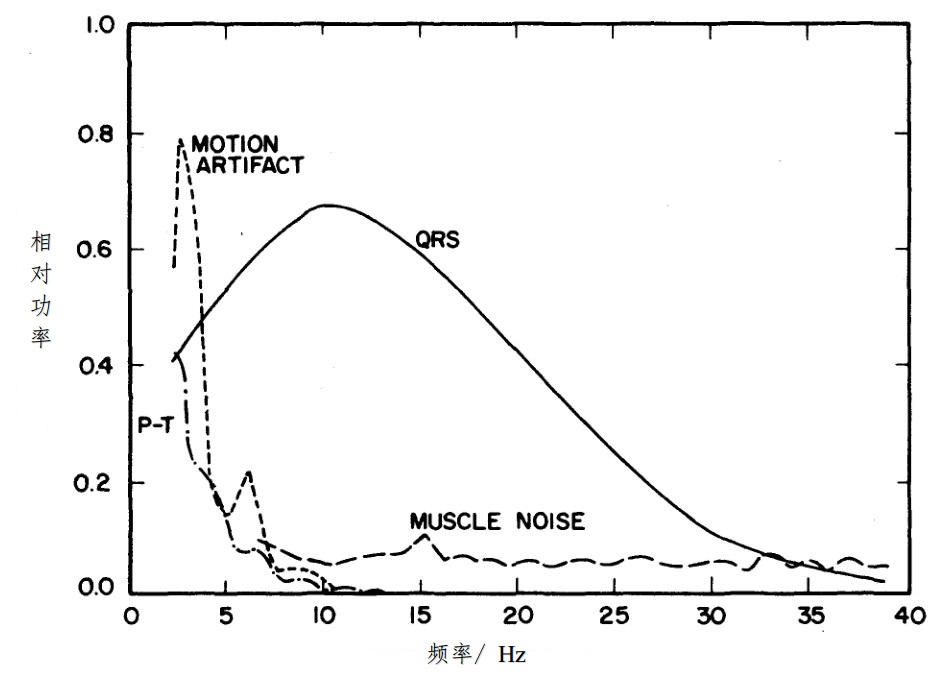
\includegraphics[width=.6\linewidth]{401}
    \caption{\label{fig:401}心电信号功率谱}
\end{figure}

由于数字滤波器的滤波精度高、算法设计灵活、可靠性高,各种基于数字滤波器的心电噪声抑制方法近年来不断涌现。 

(1) 平滑滤波器 

平滑滤波器是较早被人们采用的方法,该算法简单,处理速度快,滤波效果较好\cite{14}。其原理是基于多项式拟合方法设计的最佳简单形式的低通滤波器\cite{15}。
该方法对信号滤波时,实际上是拟合了信号中的低频成分,而将高频成分滤除。其基本的思路如下:对于信号$x(i),i=1,\dots,L$,构造一个$P$阶多项式
\begin{equation}
    \label{equ:401}
    f_i=a_0+a_1i+a_2i^{2}+\dots+a_pi^{p}
\end{equation}
以此来拟合信号。这个过程必然存在误差,设总拟合误差的平方和是 

\begin{figure}[htbp]
    \centering
    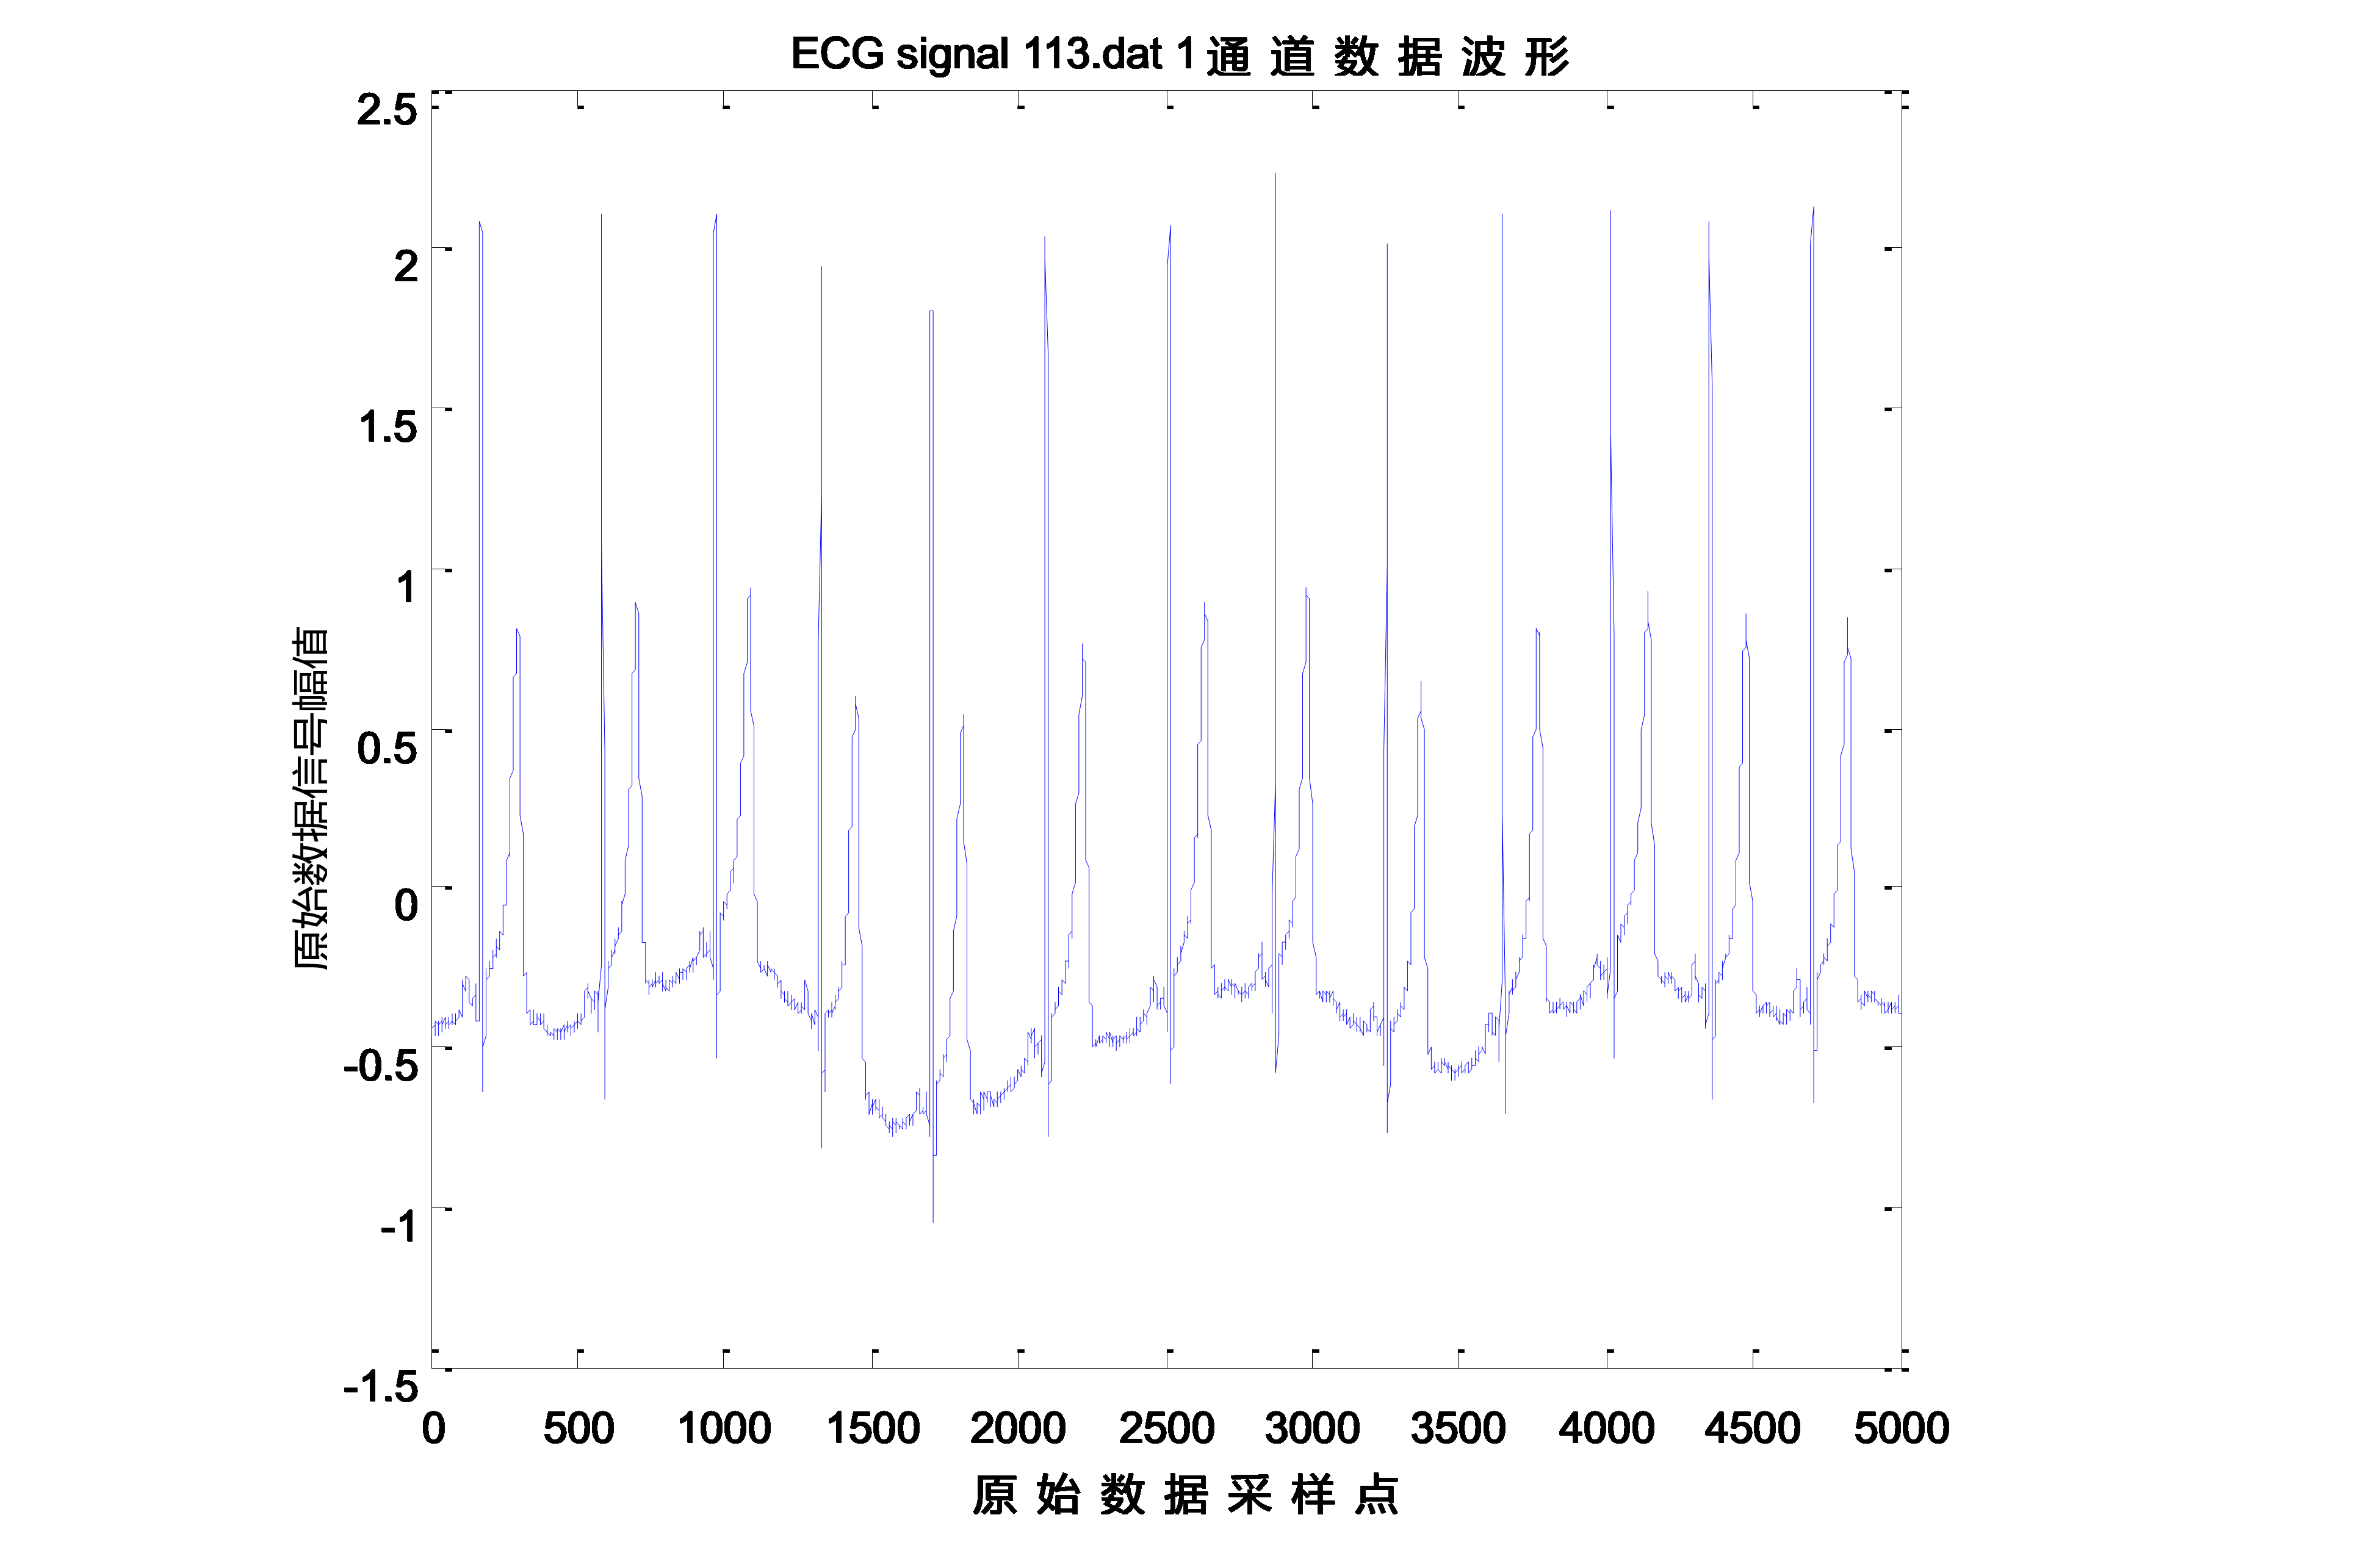
\includegraphics[width=.85\linewidth]{402}
    \caption{\label{fig:402}心电信号功率谱}
\end{figure}



\section{本章小结}
本章在前几章的基础上,实现了对实际获取的人体心电信号数据分析处理的过程,着重研究了去噪过程与信号特征提取过程的算法实现及评价上。在去噪算法模块,
着重考虑了噪声的干扰及基线漂移在心电信号检测过程中的影响,对比了平滑滤波、小波滤波及中值滤波算法的去噪效果,并在前人的基础实现了中值滤波算法的优化并在
Android 上成功移植。在特征提取方面,使用了斜率阈值的方法首先提取出了 R 波的位置,并以此为基础,依次确定了其他特征值的位置。
以上算法均在 Matlab 上进行了仿真与处理,并在 Android 上取得了基本一致的检测效果。

